%% REPLACE sXXXXXXX with your student number
\def\studentNumber{s2196789}


%% START of YOUR ANSWERS
%% Add answers to the questions below, by replacing the text inside the brackets {} for \youranswer{ "Text to be replaced with your answer." }. 
%
% Do not delete the commands for adding figures and tables. Instead fill in the missing values with your experiment results, and replace the images with your own respective figures.
%
% You can generally delete the placeholder text, such as for example the text "Question Figure 3 - Replace the images ..." 
%
% There are 5 TEXT QUESTIONS. Replace the text inside the brackets of the command \youranswer with your answer to the question.
%
% There are also 3 "questions" to replace some placeholder FIGURES with your own, and 1 "question" asking you to fill in the missing entries in the TABLE provided. 
%
% NOTE! that questions are ordered by the order of appearance of their answers in the text, and not necessarily by the order you should tackle them. You should attempt to fill in the TABLE and FIGURES before discussing the results presented there. 
%
% NOTE! If for some reason you do not manage to produce results for some FIGURES and the TABLE, then you can get partial marks by discussing your expectations of the results in the relevant TEXT QUESTIONS. The TABLE specifically has enough information in it already for you to draw meaningful conclusions.
%
% Please refer to the coursework specification for more details.


%% - - - - - - - - - - - - TEXT QUESTIONS - - - - - - - - - - - - 

%% Question 1:
\newcommand{\questionOne} {
\youranswer{According to Figure 1, the graph of loss and accuracy of VGG 38 experiment is a straight line for both training set and validation set. It represents that the model didn't learn anything after 100 epochs. However, the loss of VGG 08 experiment decreases and the accuracy of that increases as the model is trained in each iteration. By comparing Figure 2 and 3 we could find out what causes this difference. In Figure 2, the gradient flow at each layer remains in a proper range. In Figure 3, the gradient flow at deeper layer is very small, and when it back propagate to shallower layer, the gradient flow is almost 0. Hence we could conclude that the VGG 38 experiment suffers fromt the Vanishing Gradient Problem.  }
}

%% Question 2:
\newcommand{\questionTwo} {
\youranswer{Batch Normalization (BN) uses trainable parameters 
to normalize the input hidden units of each layer. The specific process of how BN works involves with the following equation. Firstly we need to calculate the mean and varaince for a given minibatch:

\begin{equation}
    \label{eq.mean}
    \mu_i \longleftarrow \dfrac{1}{M}\sum_{m=1}^{M}u_i^{m}
\end{equation}

\begin{equation}
    \label{eq.var}
    \sigma_i^2 \longleftarrow  \dfrac{1}{M}\sum_{m=1}^{M}(u_i^m-\mu_i)^2
\end{equation}

After we got the mean and variance for the certain minibatch, we need to this minibatch using the mean and variance we calculated above:

\begin{equation}
    \label{eq.norm}
    \hat{u_i}=\dfrac{u_i-\mu_i}{\sqrt{\sigma_i^2+\epsilon}}
\end{equation}

If we just normalize the bath using the above equation without doing anything else, the neural network won't learn anything from this. The most important thing is that we need to add two learnable parameters $\gamma$ and $\beta$ to scale and shift each instance of the minibatch to make the BN nonlinear.

\begin{equation}
    \label{eq.bn}
    z^i=\gamma_i\hat{u_i}+\beta_i
\end{equation}

At training time we set $\gamma$ and $\beta$ by gradient descent which requires $\gamma$ and $\beta$ differentiable with respect to the loss function. And we will upgrade those values in back propagation using $\dfrac{\partial E}{\partial \hat{u}}$, $\dfrac{\partial E}{\partial \sigma^2}$, $\dfrac{\partial E}{\partial \mu}$ and $\dfrac{\partial E}{\partial u_i}$. At test time the minibatch is normalized at each layer using parameters computed over the complete training data. BN could effectively increase training speed by making the gradient of input of each layer unsaturated and increasing speed of convergence.}
}

%% Question 3:
\newcommand{\questionThree} {
\youranswer{ Residual Connections (RC) is composed of two kind of mapping, identity mapping and residual mapping. In a block of Residual Connection, the identity mapping creates a shortcut connection from the input of a convolutional layer to before the final activation function of that block. The following equation shows what residual learning does in a RC block.

\begin{equation}
    \label{eq.bn}
    y = F(x,{W_i})+x
\end{equation}

The component $x$ is the identity mapping, while $F(x,{W_i})$ is the residual mapping which is the difference between the mapping of convolutional layer and its input $x$. The residual mapping and the identity mapping are added based on element-wise operation . Hence the dimension of their channel must be the same. For different dimension of channels, we could add an additional convectional layer:

\begin{equation}
    \label{eq.bn}
    y = F(x,{W_i})+W_sx
\end{equation}

RC could alleviate the problem of gradient vanishing because it allows the learnt features of shallower layer propagate to deeper layer to get rid of accuracy degradation on deeper layers. During training time the residual mapping is trained until the model is optimal, and the identity mapping ensures the whole neural network being optimal all the time.}
}

%% Question 4:
\newcommand{\questionFour} {
\youranswer{After we implementing both BN and RC to VGG38 model we could find that there is a significant improving on its accuracy and loss. In experiment of BN+RC, we implemented BN on both processing blocks and reduction blocks, and we implemented RC only on processing blocks. By comparing Figure\ref{fig:grad_flow_38} and Figure\ref{fig:grad_flow_bestModel} which shows gradient flow on VGG38 with and without BN+RC, we could find that the gradient flow model implemented with BN and RC is much better and there is no longer gradient vanishing problem anymore. Figure\ref{fig:curves} shows that the accuracy and loss per epoch is much better than the broken neurol network. The accuracy is increasing and the loss is decreasing through each iteration of training.

Moreover, there are some noticeable points according to the experiment results table\ref{tab:CIFAR_results}. Implementing both BN and RC individually on VGG38 model also helps improving its performance, while RC has better performance than BN. On the same learning rate, the combination of BN and RC has the highest training/validation accuracy and the lowest loss, which tells us implementing BN and RC together will give us the best performance. In addition, the model with learning rate of 1e-3 has generally high accuracy than that with learning rate of 1e-2.

By looking at parameters of each model, We could also find that the model implementing with BN has more parameters than that without BN. The difference is because BN adds some additional learnable parameters to normalize the input hidden units of each layer. The more layers in a neural network, the more trainable parameters to be added. We could furthermore run experiments with more layers and number of blocks at each stage and test the performance of BN and RC individually to see how they alleviate the problem of vanishing gradient on deeper neural network comparing with the models on table\ref{tab:CIFAR_results}. We could also implement them on shallower neural network such as VGG08 to see if they helps improving its accuracy or not. Changing the learning rate also affects the performance of model and hence it's worthy to try a different list of learning rate.}
}

%% Question 5:
\newcommand{\questionFive} {
\youranswer{In general, the best model in these combinations of VGG08, VGG38, BN, RC and LR we discussed is VGG38 BN+RC with learning rate of 1e-3. The performance of the model trained could also be improved by adjusting the hyperparmeters of learning rate. Our experiments confirms the effectiveness of BN and RC on resolving problem of gradient vanishing and significant improvement on the accuracy of VGG38 comparing with the broken neural network. From this experiment we evidenced how BN and RC work and the theory behind why they would work. However, we need to do further experiments to test BN and RC on different neural networks with different layers. Whether BN and RC work at the same performance on deeper neural networks still needs to be examined.}
}

%% - - - - - - - - - - - - FIGURES - - - - - - - - - - - - 

%% Question Figure 3:
\newcommand{\questionFigureThree} {
\youranswer{
%
\begin{figure}[t]
    \centering
    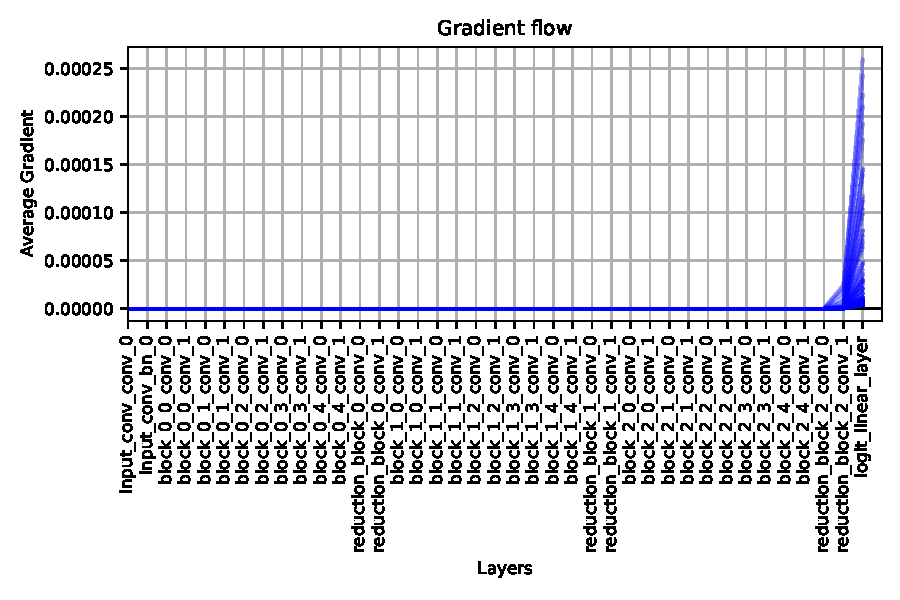
\includegraphics[width=\linewidth]{figures/grad_flow_vgg38.pdf}
    \caption{Gradient Flow on VGG38}
    \label{fig:grad_flow_38}
\end{figure}
}
}

%% Question Figure 4:
\newcommand{\questionFigureFour} {
\youranswer{
%
\begin{figure}[t]
    \begin{subfigure}{\linewidth}
        \centering
        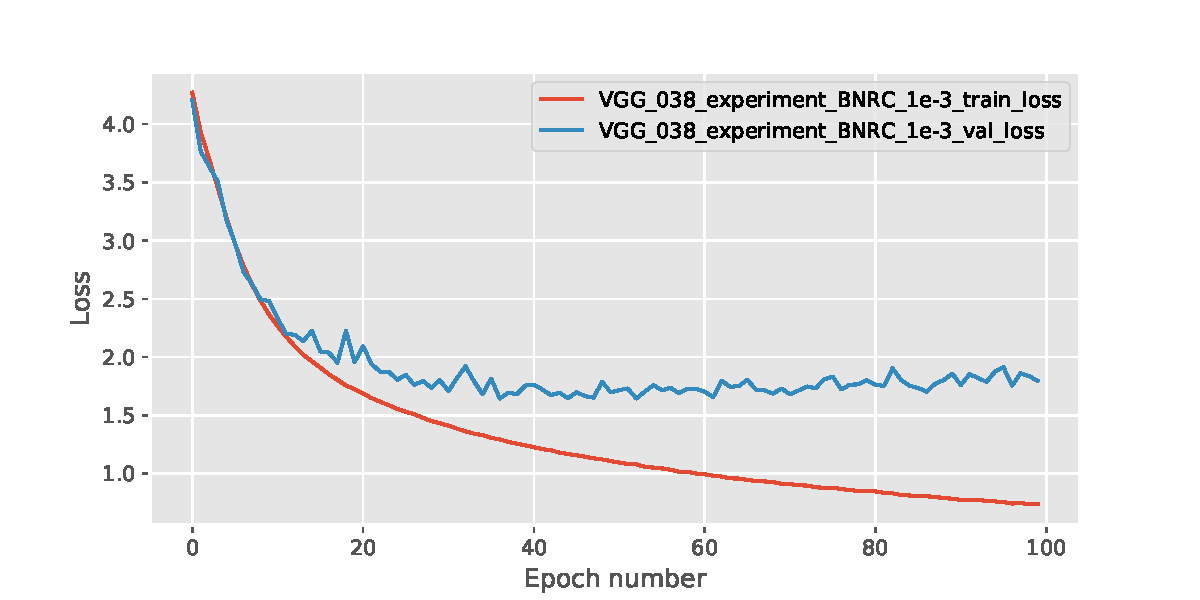
\includegraphics[width=\linewidth]{figures/best_model_loss_performance.pdf}
        \caption{Loss per epoch}
        \label{fig:loss_curves}
    \end{subfigure}

    \begin{subfigure}{\linewidth}
        \centering
        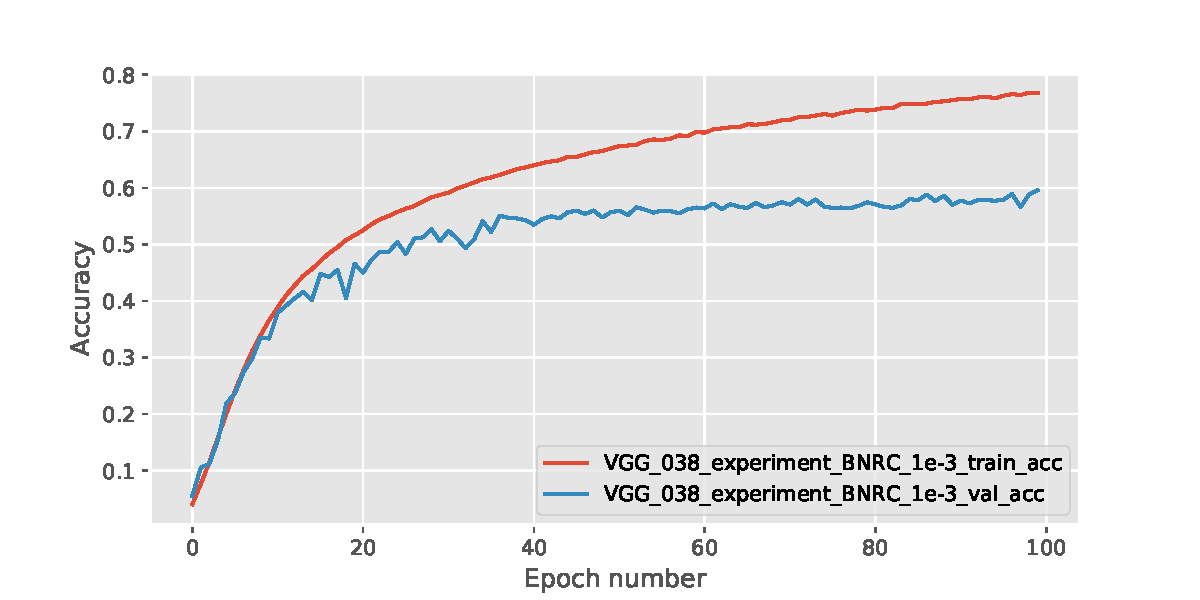
\includegraphics[width=\linewidth]{figures/best_model_accuracy_performance.pdf}
        \caption{Accuracy per epoch}
        \label{fig:acc_curves}
    \end{subfigure}
    \caption{Training curves for VGG38 BN+RC LR1e-3}
    \label{fig:curves}
\end{figure}
}
}

%% Question Figure 5:
\newcommand{\questionFigureFive} {
\youranswer{
%
\begin{figure}[t]
    \centering
    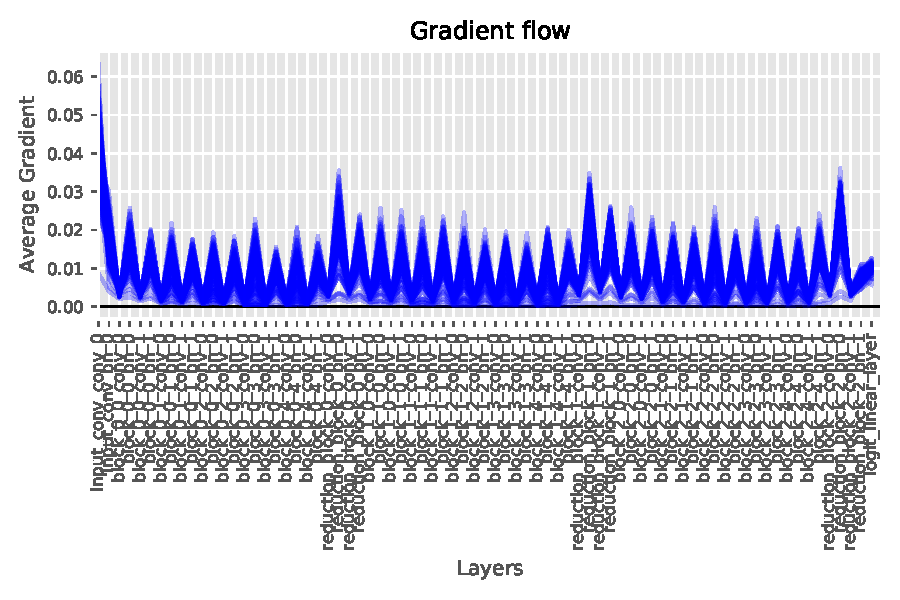
\includegraphics[width=\linewidth]{figures/grad_flow_best.pdf}
    \caption{Gradient Flow on VGG38 BN+RC LR1e-3}
    \label{fig:grad_flow_bestModel}
\end{figure}
}
}

%% - - - - - - - - - - - - TABLES - - - - - - - - - - - - 

%% Question Table 1:
\newcommand{\questionTableOne} {
\youranswer{
%
\begin{table*}[t]
    \centering
    \begin{tabular}{lr|ccccc}
    \toprule
        Model                   & LR   & \# Params & Train loss & Train acc & Val loss & Val acc \\
    \midrule
        VGG08                   & 1e-3 & 60 K    &  1.74      & 51.59     & 1.95     & 46.84 \\
        VGG38                   & 1e-3 & 336 K   &  4.61      & 00.01     & 4.61     & 00.01 \\
        VGG38 BN                & 1e-3 & 339 K   &  1.47      & 57.94     & 1.88     & 48.60 \\
        VGG38 RC                & 1e-3 & 336 K   &  1.33      & 61.52     & 1.84     & 52.32 \\
        VGG38 BN + RC           & 1e-3 & 339 K   &  0.74      & 76.76     & 1.79     & 59.56 \\
        VGG38 BN                & 1e-2 & 339 K   &  1.75      & 50.73     & 2.01     & 45.84 \\
        VGG38 BN + RC           & 1e-2 & 339 K   &  0.72      & 76.86     & 1.86     & 57.60  \\
    \bottomrule
    \end{tabular}
    \caption{Experiment results (number of model parameters, Training and Validation loss and accuracy) for different combinations of VGG08, VGG38, Batch Normalisation (BN), and Residual Connections (RC), LR is learning rate.}
    \label{tab:CIFAR_results}
\end{table*} 
}
}

%% END of YOUR ANSWERS